\chapter{\IfLanguageName{dutch}{integratie van localisatie technologieën}{Integration of Localization Technologies}}%
\label{ch:localisatie}

\subsection{Doelstelling}
Deze fase was gericht op het integreren van geavanceerde locatietechnologieën om de exacte GPS-locaties van de koeien in het veld te bepalen door middel van cameraperspectieftransformatie. Het doel was om de nauwkeurigheid van de locatiegegevens te verhogen en real-time tracking van koeien op het veld mogelijk te maken.

\subsection{Methoden}
\begin{itemize}
  \item \textbf{Camera Perspective Transformation:}
  \begin{itemize}
    \item \textbf{Camera Intrinsics en Extrinsics:} Voor de implementatie van de locatiebepaling werd gebruik gemaakt van de intrinsieke (zoals de lensspecificaties) en extrinsieke (zoals de oriëntatie en positie ten opzichte van het veld) eigenschappen van de camera. Deze gegevens zijn essentieel voor het nauwkeurig omzetten van pixelcoördinaten in het beeld naar echte wereldcoördinaten op het veld.
    \item \textbf{Veld Kalibratie:} De vier hoeken van het veld werden in het camerabeeld gemarkeerd en gekoppeld aan de corresponderende GPS-locaties. Deze kalibratie maakte het mogelijk om de locatie van elk punt binnen het veld nauwkeurig te berekenen door de pixelpositie in het camerabeeld om te zetten naar een GPS-locatie.
  \end{itemize}
  \item \textbf{Nauwkeurigheidstests:}
  \begin{itemize}
    \item \textbf{Veldtests met een nepkoe:} Om de nauwkeurigheid van het systeem te verifiëren, werden experimenten uitgevoerd waarbij een nepkoe op verschillende locaties en in verschillende oriëntaties op het veld werd geplaatst. Voor elke positie werd de exacte GPS-locatie geregistreerd met behulp van een Emlid Reach Rs3 RTK GPS tracker, die bekend staat om zijn hoge nauwkeurigheid met een precisie tot op 1 cm in vaste positie.
    \newline 
    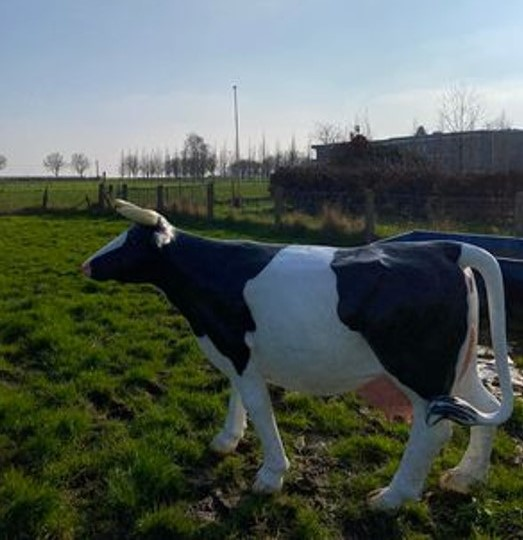
\includegraphics[width=0.7\linewidth]{localisatie_nepkoe.jpg}
    \newline 
    \item \textbf{Analyse van Foutmarges:} De initiële tests toonden een foutmarge van 0 tot 3 meter. Een consistente kleine foutmarge werd veroorzaakt door lichte bewegingen van de camera als gevolg van de wind. Deze fout bleek consistent in dezelfde richting te zijn, waardoor het mogelijk werd om de gemiddelde fout van de metingen af te trekken en zo de nauwkeurigheid van de camera-gebaseerde GPS-locaties te verbeteren tot een maximale foutmarge van 30 cm. Plannen voor het toepassen van beeldstabilisatie in de volgende fase zijn opgesteld om deze kleine bewegingen te compenseren.
    \item \textbf{Plot effectieve gps locaties:} 
    \newline 
    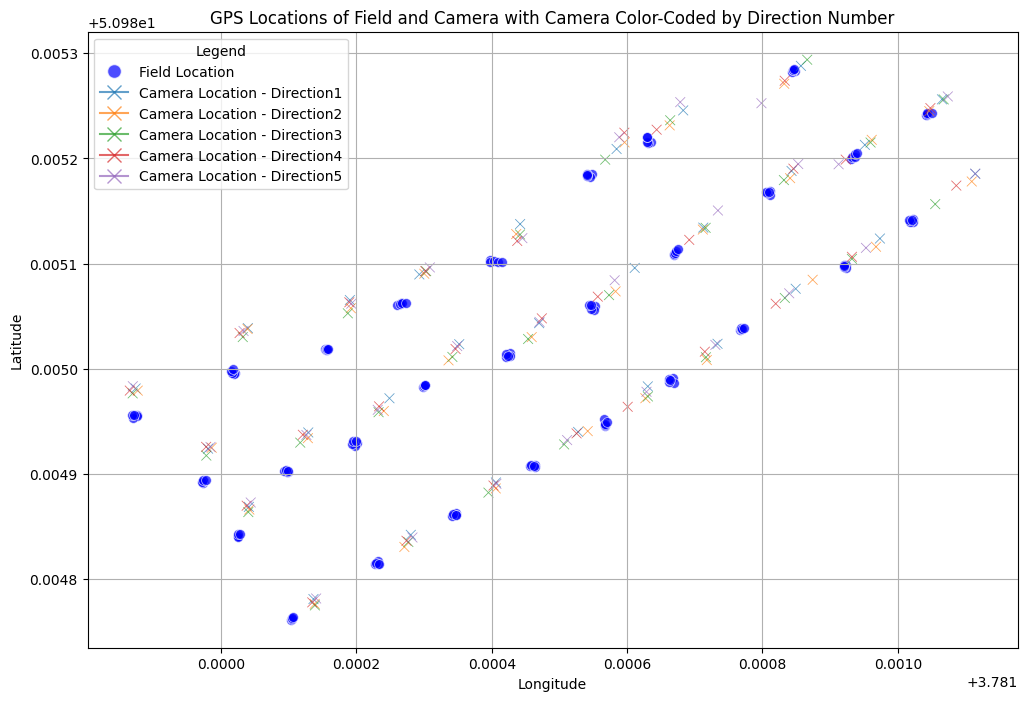
\includegraphics[width=\linewidth]{localisatie_plot_effectivelocations.png}
    \newline 
    \item \textbf{Plot gecorigeerde gps locaties:} 
    \newline
    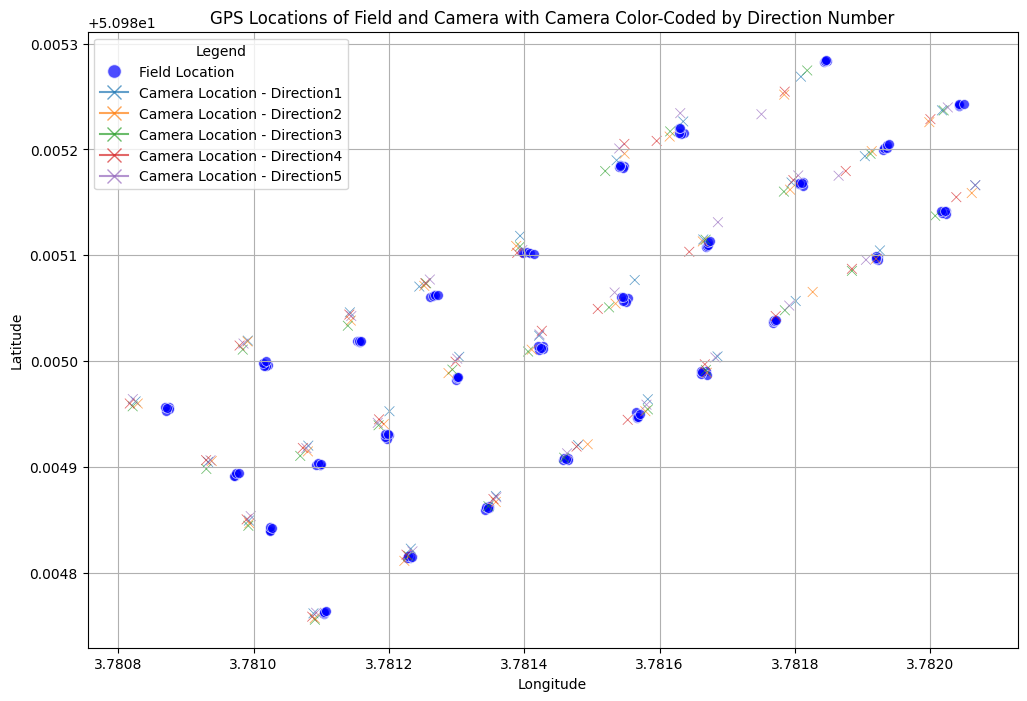
\includegraphics[width=\linewidth]{localisatie_plot_corrected_fault.png}
    \newline 
  \end{itemize}
\end{itemize}

\subsection{Resultaten}
\begin{itemize}
  \item \textbf{Geïmplementeerde Technologie:} De ontwikkelde techniek voor het bepalen van GPS-locaties via cameraperspectieftransformatie is succesvol geïmplementeerd en getest, wat heeft geleid tot een betrouwbare methode voor het real-time volgen van koeien op het veld.
  \item \textbf{Invloed van Rotatie:} Uit de analyses bleek dat de rotatie van de koe geen significante invloed had op de richting of afstand van de GPS-locaties, wat de robuustheid van het systeem bevestigt. 
  \newline 
  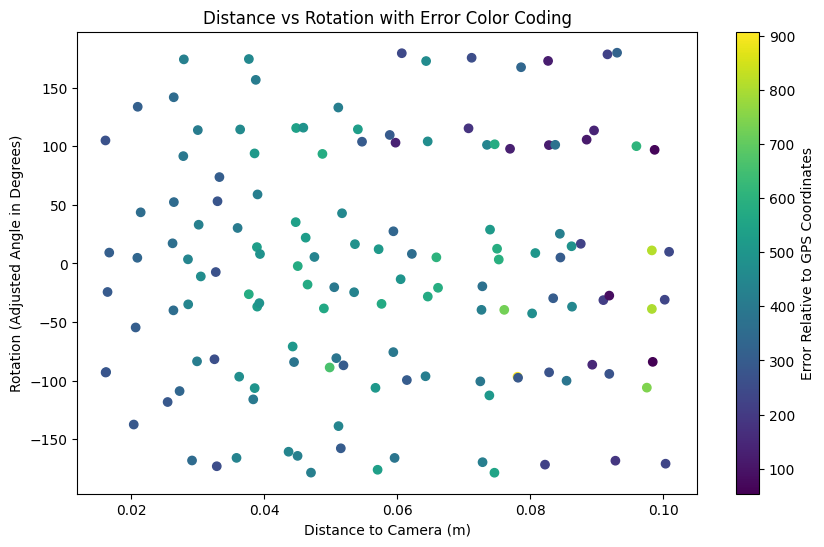
\includegraphics[width=\linewidth]{localisation_rotation_fault.png}
  \newline
  \item \textbf{Visualisatie en Evaluatie:} De resultaten van de locatiebepaling zijn gevisualiseerd en beoordeeld, waarbij de effectiviteit van de techniek werd bevestigd. Deze geavanceerde locatietechniek biedt aanzienlijke verbeteringen ten opzichte van traditionele niet-RTK GPS-sensoren, die doorgaans een foutmarge van ongeveer 3 meter hebben.
\end{itemize}